
\documentclass[fleqn,addpoints]{exam}
\usepackage{amsmath}
\usepackage{graphicx}
\usepackage{booktabs}
\usepackage{float}
\usepackage{caption}
\usepackage{polynom}
\usepackage{mdwlist}
\usepackage{cancel}

\usepackage{unitsdef} 
\newunit{\inch}{in}
\newunit{\mile}{mile}
\newunit{\mph}{mph}
\newunit{\foot}{ft}
\newunit{\knot}{knot}
\newunit{\gallon}{gallon}

\bracketedpoints
\everymath{\displaystyle}

\printanswers

\ifprintanswers 
\usepackage{2in1, lscape} 
\fi

% \begin{figure}[H]
%   \centering
%   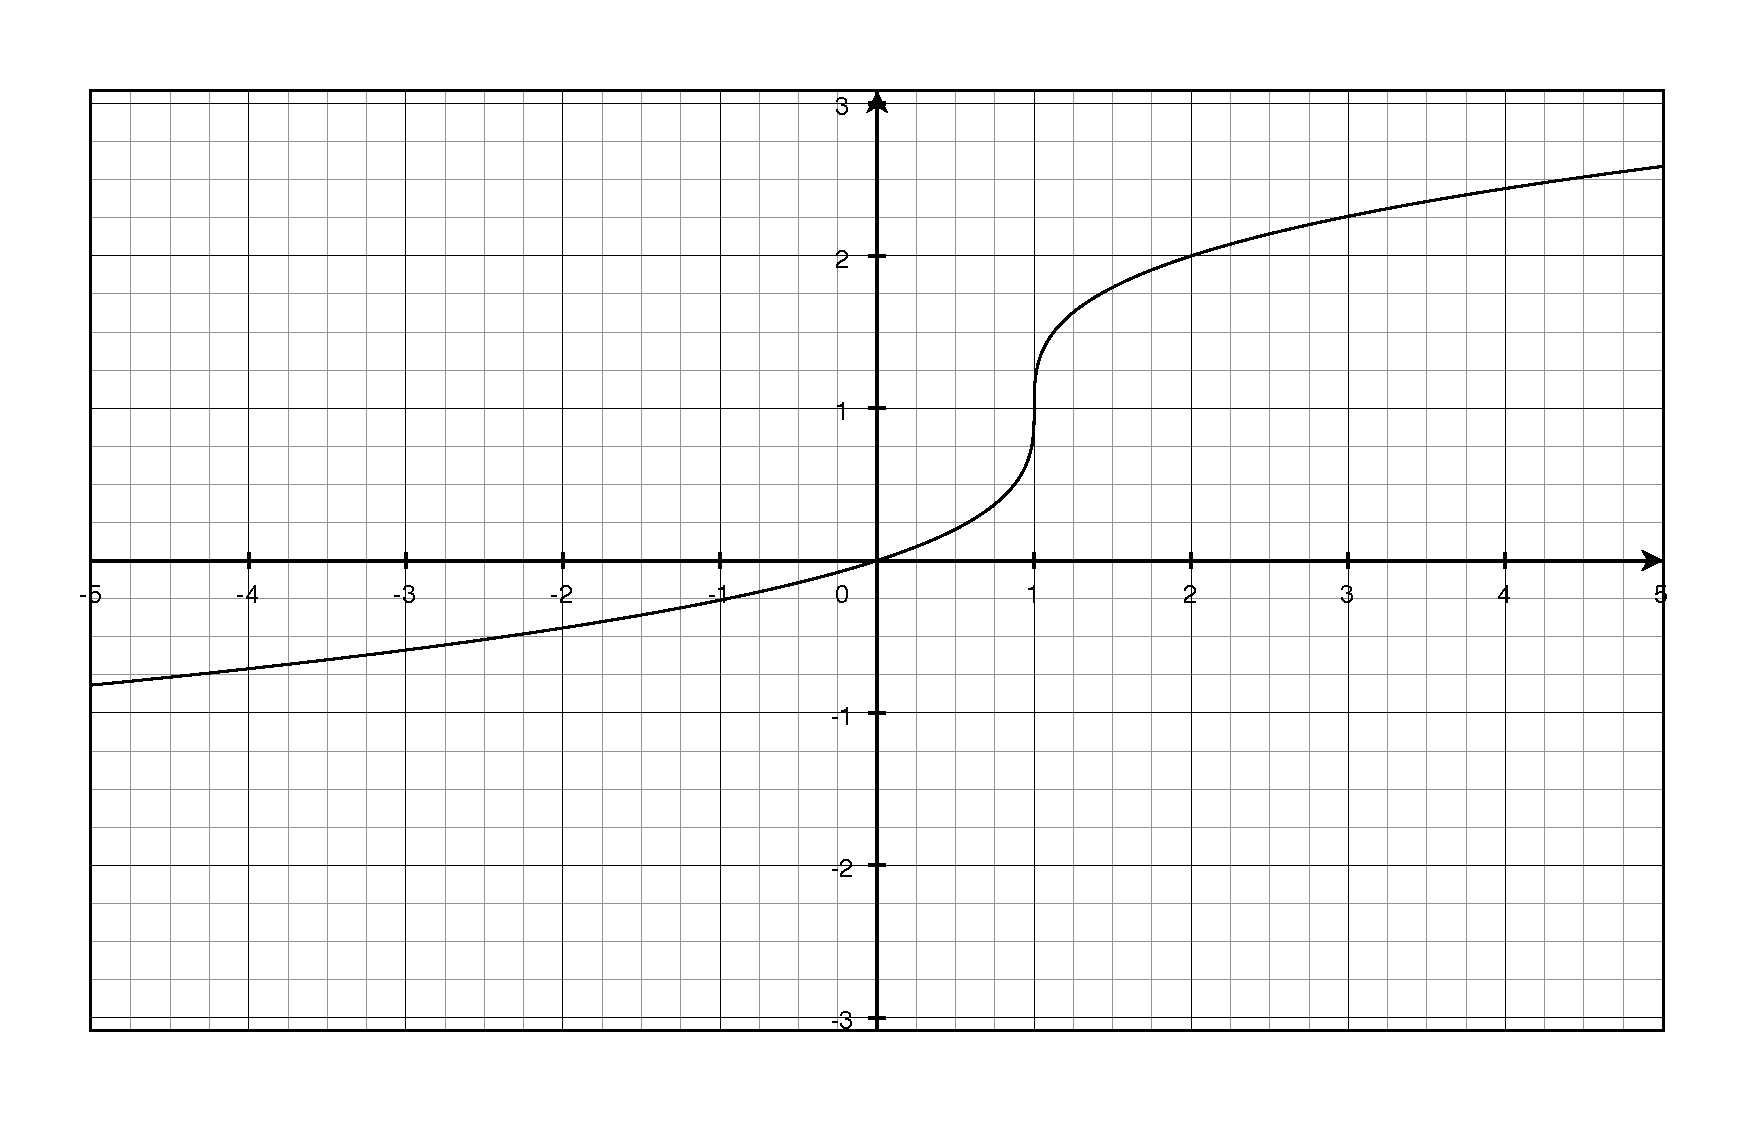
\includegraphics[scale=.3]{question7.eps}
%   \caption*{Question 7}
% \end{figure}

% \begin{tabular}{cc}
% \toprule
% period & amplitude \\
% \midrule
%   $\pi$ & $2$ \\
% \bottomrule
% \end{tabular}


%% \ifprintanswers
%% \usepackage{2in1, lscape}
%% \fi

\title{Math 263A Sample Final Exam One}
\date{October 18, 2012}

\author{}

\begin{document}

\maketitle  

\begin{questions}

\question The edge of a cube is found to be 30 cm with a maximum error in measurement of 0.3 cm. Use differentials to
estimate the maximum possible error in computing:

\begin{parts}
\part the volume of the cube
\begin{solution}
\begin{align*}
  V &= x^3 \\
  dV &= 3x^2 \, dx \\
     &= 3 \cdot 30^2 \cdot 0.3 \centimeter^3 \\
     &= 810 \ \centimeter^3 \\
\end{align*}  
\end{solution}

\part the surface area of the cube.
\begin{solution}
\begin{align*}
  A &= 6 x^2 \\
  dA &= 12x \, dx \\
     &= 12 \cdot 30 \cdot 0.3 \centimeter^2 \\
     &= 108 \ \centimeter^2 \\
\end{align*}  
\end{solution}

\end{parts}

\question If $y = x^3 + y^3$, find $\frac{dy}{dx}$ and $\frac{d^2y}{dx^2}$ by implicit differentiation.

\begin{solution}
\begin{align*}
  y &= x^3 + y^3 \\
  y' &= 3x^2 + 3y^2y' \\
  y' - 3y^2y' &= 3x^2 \\
  y' &= \frac{3x^2}{1 - 3y^2} \\
\\
  y'' &= \frac{(1 - 3y^2)(6x) - 3x^2(-6yy')}{(1 - 3y^2)^2} \\
   &= \frac{6x}{1 - 3y^2} + \frac{18x^2yy'}{(1 - 3y^2)^2} \\
   &= \frac{6x}{1 - 3y^2} + \frac{54x^4y}{(1 - 3y^2)^3} \\
\end{align*}

\end{solution}

\ifprintanswers
\pagebreak
\fi

\question $f(x)= \sqrt{x - 1}$
\begin{parts}
\part Find $f'(x)$ using the definition of derivative. 

\begin{solution}
\begin{align*}
  f'(x) &= \lim_{h \to 0} \frac{\sqrt{x - 1 + h} - \sqrt{x - 1}}{h} \\
  &= \lim_{h \to 0} \frac{\sqrt{x - 1 + h} - \sqrt{x - 1}}{h} \cdot \frac{\sqrt{x - 1 + h} + \sqrt{x - 1}}{\sqrt{x - 1 + h} + \sqrt{x - 1}} \\
  &= \lim_{h \to 0} \frac{\cancel{h}}{\cancel{h} \left( \sqrt{x - 1 + h} + \sqrt{x - 1} \right)} \\
  &= \lim_{h \to 0} \frac{1}{\sqrt{x - 1 + h} + \sqrt{x - 1}} \\
  &= \frac{1}{2 \sqrt{x - 1}} \\
\end{align*}

\end{solution}

\part State the domains of $f(x)$ and $f'(x)$.
\begin{solution}
The domain of $f$ is $[1, \infty)$ and the domain of $f'$ is $(1, \infty)$
\end{solution}

\end{parts}

\question
\begin{parts}

\part If $A(r)$ is the area of a circle with radius $r$ and the circle expands as time passes, find
$\frac{dA}{dt}$ in terms of $\frac{dr}{dt}$. 

\begin{solution}
\begin{align*}
  A &= \pi r^2 \\
  \frac{dA}{dt} &= 2 \pi r \cdot \frac{dr}{dt} \\  
\end{align*}
\end{solution}

\part Suppose oil spills from a ruptured tanker and spreads in a circular pattern. If the radius of the oil spill
increases at a constant rate of 1 m/s, how fast is the area of the spill increasing when the radius is 30 m?

\begin{solution}
\begin{align*}
  \frac{dA}{dt} &= 2 \pi r \cdot \frac{dr}{dt} \\  
  &= 2 \pi \cdot (30 \meter)(1 \meter / \second) \\
  &= 60 \pi \meter^2 / \second \\
\end{align*}

\end{solution}

\end{parts}

\question
Find the derivative of: $f(x) = \sqrt{\frac{x^2 + 1}{x^2 - 1}}$

\begin{solution}
\begin{align*}
  f(x) &= \left( \frac{x^2 + 1}{x^2 - 1} \right) \\
  f'(x) &= \frac{1}{2} \left( \frac{x^2 + 1}{x^2 - 1} \right)^{-1/2} 
               \cdot \frac{(x^2 - 1)(2x) - (x^2 + 1)(2x)}{(x^2 + 1)^2} \\
    &= \frac{1}{2} \frac{(x^2 - 1)^{1/2}}{(x^2 + 1)^{1/2}} \cdot \frac{-4x}{(x^2 + 1)^2} \\
    &= - \frac{2x (x^2 - 1)^{1/2}}{(x^2 + 1)^{5/2}}
\end{align*}

\end{solution}

\question
If $1,200 \ \cm^2$ of material is available to make a box with a square base and an open top, find the largest possible volume
of the box.

\begin{solution}
If $h$ is the height and $x$ is the length of a side, the two equations for the box are:
\begin{align*}
  A &= x^2 + 4xh \\
  V &= x^2h \\
\end{align*}
We want to maximize the volume, but the volume equation has too many variables.  Since the area is fixed, we can solve the area equation
for the height in terms of the area and plug that into the volume equation.
\begin{align*}
  A &= x^2 + 4xh \\
  h &= \frac{A}{4x} - \frac{x}{4} \\
\\
  V &= x^2 \left( \frac{A}{4x} - \frac{x}{4} \right) \\
    &= \frac{Ax}{4} - \frac{x^3}{4} \\
\end{align*}
Now we can differentiate the volume equation to find the maximum point:
\begin{align*}
   V &= \frac{Ax}{4} - \frac{x^3}{4} \\
   \frac{dV}{dx} &= \frac{A}{4} - \frac{3x^2}{4} \\
\\
   0 &= \frac{A}{4} - \frac{3x^2}{4} \\
%   3x^2 &= A \\
   x &= \sqrt{\frac{A}{3}} \\
     &= \sqrt{\frac{1200}{3}} \cm \\
     &= 20 \cm \\
\end{align*}
Now we can plug $x$ into the height equation to find the height:
\begin{align*}
    h &= \frac{A}{4x} - \frac{x}{4} \\
      &= \frac{1200}{80} - \frac{20}{4} \cm \\
      &= 10 \cm \\
\end{align*}

So the best dimensions are a box with a height of $10 \cm$ and a base with $20 \cm$ sides giving a total volume of 
$4000 \cm^3$.  

It makes sense that the height is smaller than the length of the sides of the base.  There are
4 sides and only 1 base, so you'll want to make the sides smaller than the base.


\end{solution}

\question $V(r) = 4 \pi r^3$; $[0, 3]$.
\begin{parts}
\part Differentiate $V$
\begin{solution}
\[
  V'(r) = 12 \pi r^2
\]
\end{solution}

\part Verify that $V$ satisfies the hypotheses of the Mean Value Theorem on the given interval.  Then find all numbers
$c$ that satisfy the conclusion of the Mean Value Theorem.

\begin{solution}
Since $V$ is a polynomial, it is continuous everywhere.

\[
  V_{avg} = \frac{V(3) - V(0)}{3} = 36 \pi
\]

\begin{align*}
  12 \pi r^2 &= 36 \pi \\
  r &= \sqrt{3} \\
\end{align*}

\end{solution}

\end{parts}

\ifprintanswers
\pagebreak
\fi

\question Find the constant $c$ that makes $g$ continuous on $(-\infty, \infty)$.
\[
  g(x) = \bigg\{ \frac{x^2 - c^2 \text{ if } x \leq 4}{cx + 20 \text{ if } x \geq 4}
\]

\begin{solution}
For the function to be continuous, the two equations must be equal at $x = 4$.
\begin{align*}
  4^2 - c^2 &= 4c + 20 \\
  c^2 + 4c + 4 &= 0 \\
  (c + 2)^2 &= 0 \\
  c &= -2 \\
\end{align*}

\end{solution}

\question $f(x) = 3x^2 - 12x + 5$.  Find the maximum and minimum values of $f$ on $[0, 3]$.
\begin{solution}
\begin{align*}
  f(x) &= 3x^2 - 12x + 5 \\
  f'(x) &= 6x - 12 \\
  6x - 12 &= 0 \\
  x &= 2 \\
\end{align*}

\begin{center}
\begin{tabular}{rr}
\toprule
$x$ & $f(x)$ \\
\midrule
  0 & $5$ \\
  2 & $-7$ \\
  3 & $-4$ \\
\bottomrule
\end{tabular}
\end{center}

The minimum value is $(2, -7)$ and the maximum value is $(0, 5)$.

\end{solution}

\pagebreak

\question $f(x) = 2x^3 - 3x^2 - 12x$
\begin{parts}
\part \label{graph:first} Find the vertical and horizontal asymptotes.
\begin{solution}
  Since $f$ is a polynomial, there aren't any asymptotes.
\end{solution}

\part Find the intervals on which f is increasing or decreasing. 

\begin{solution}
\begin{align*}
  f'(x) &= 6x^2 - 6x - 12 \\
\\
  6x^2 - 6x - 12 &= 0 \\
  x^2 - x - 2 &= 0 \\
  (x - 2)(x + 1) &= 0 \\
  x &= \{-1, 2\} \\
\end{align*}

With a sign chart or test points, you can find that $f$ is:
\begin{itemize*}
\item increasing: $(-\infty, -1) \cup (2, \infty)$
\item decreasing: $(-1, 2)$
\end{itemize*}
  
\end{solution}

\part Find the local maximum and minimum values of $f$.
\begin{solution}
\begin{itemize*}
\item local max: $(-1, 7)$
\item local min: $(2, -20)$
\end{itemize*}
\end{solution}

\ifprintanswers
\pagebreak
\fi

\part \label{graph:last} Find the intervals of concavity and the inflection points. 
\begin{solution}
\begin{align*}
  f''(x) &= 12x - 6 \\
\\
  12x - 6 &= 0 \\
  x &= \frac{1}{2} \\
\end{align*}

With a sign chart or test points, you can find that $f$ is:
\begin{itemize*}
\item concave up: $\left[\frac{1}{2}, \infty \right)$
\item concave down: $\left(-\infty, \frac{1}{2} \right]$
\end{itemize*}

\end{solution}

\part Use the information from (\ref{graph:first}) to (\ref{graph:last}) to sketch the graph.
\begin{solution}
\begin{figure}[H]
  \centering
  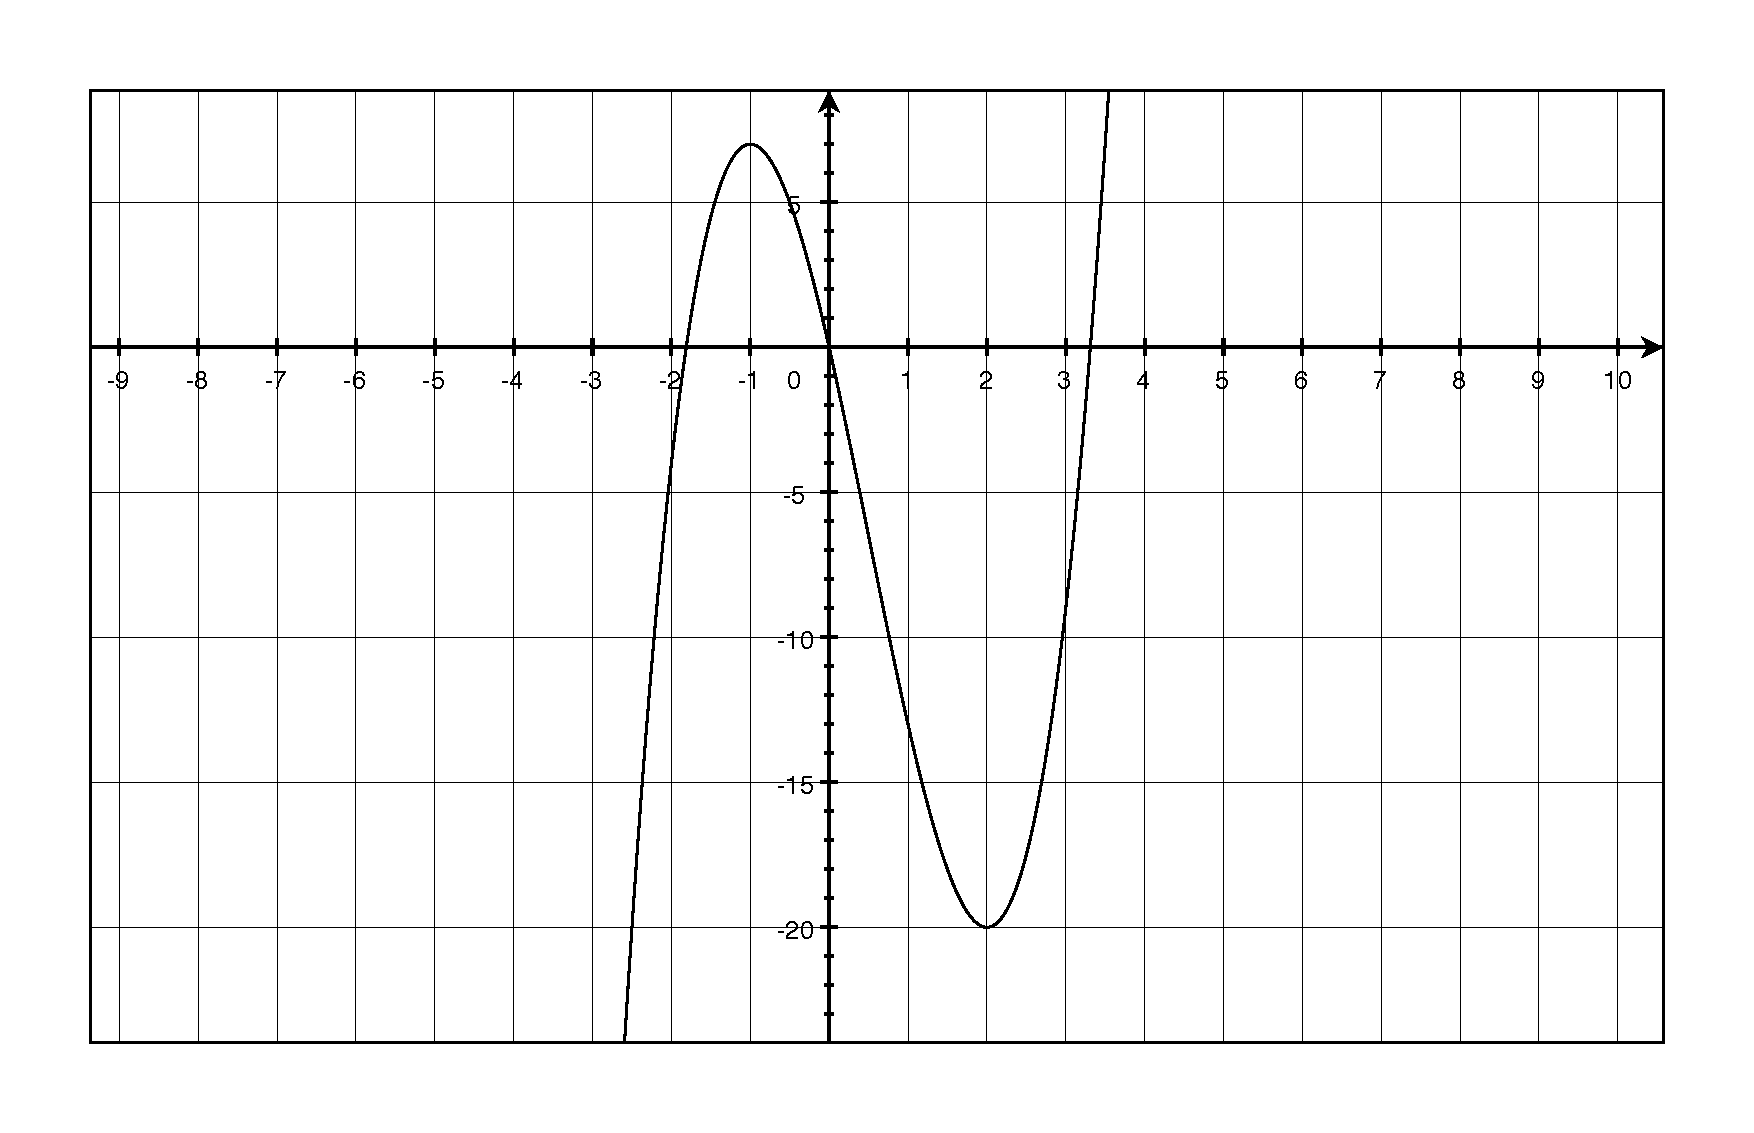
\includegraphics[scale=.3]{final_1_q10.eps}
  \caption*{Question 10}
\end{figure}
\end{solution}

\end{parts}

\question
Evaluate the limit:
\[
  \lim_{x \to \frac{\pi}{2}^+} \frac{\cos x}{1 - \sin x}
\]

\begin{solution}
\begin{align*}
  \lim_{x \to \frac{\pi}{2}^+} \frac{\cos x}{1 - \sin x} &=
    \lim_{x \to \frac{\pi}{2}^+} \frac{\cos x}{1 - \sin x} \cdot \frac{1 + \sin x}{1 + \sin x} \\
  &= \lim_{x \to \frac{\pi}{2}^+} \frac{\cos x (1 + \sin x)}{1 - \sin^2 x} \\
  &= \lim_{x \to \frac{\pi}{2}^+} \frac{\cos x (1 + \sin x)}{\cos^2 x} \\
  &= \lim_{x \to \frac{\pi}{2}^+} \frac{(1 + \sin x)}{\cos x} \\
  &= - \infty \\  
\end{align*}

The answer is negative because of the direction by which $x$ is approaching the limit.  When $x > \frac{\pi}{2}$, 
 $\cos x$ is negative and approaching 0 while $1 + \sin x$ is approaching 2.
\end{solution}



\question
Find the derivative:
\[
  y = \frac{1}{x^2} + x \cos x
\]

\begin{solution}
\begin{align*}
  y &= x^{-2} + x \cos x \\
  y' &= -2x^{-3} + x \cdot (- \sin x) + \cos x \\
     &= - \frac{2}{x^3} - x \sin x + \cos x \\
\end{align*}
  
\end{solution}

\end{questions}

\end{document}
